%iffalse%\let\negmedspace\undefined
\let\negthickspace\undefined
\documentclass[journal,12pt,onecolumn]{IEEEtran}
\usepackage{cite}
\usepackage{amsmath,amssymb,amsfonts,amsthm}
\usepackage{algorithmic}
\usepackage{graphicx}
\usepackage{textcomp}
\usepackage{xcolor}
\usepackage{txfonts}
\usepackage{listings}
\usepackage{enumitem}
\usepackage{mathtools}
\usepackage{gensymb}
\usepackage{comment}
\usepackage[breaklinks=true]{hyperref}
\usepackage{tkz-euclide} 
\usepackage{listings}
\usepackage{gvv}                                        
%\def\inputGnumericTable{}                                 
\usepackage[latin1]{inputenc}     
\usepackage{xparse}
\usepackage{color}                                            
\usepackage{array}                                            
\usepackage{longtable}                                       
\usepackage{calc}                                             
\usepackage{multirow}
\usepackage{multicol}
\usepackage{hhline}                                           
\usepackage{ifthen}                                           
\usepackage{lscape}
\usepackage{tabularx}
\usepackage{array}
\usepackage{float}
\newtheorem{theorem}{Theorem}[section]
\newtheorem{problem}{Problem}
\newtheorem{proposition}{Proposition}[section]
\newtheorem{lemma}{Lemma}[section]
\newtheorem{corollary}[theorem]{Corollary}
\newtheorem{example}{Example}[section]
\newtheorem{definition}[problem]{Definition}
\newcommand{\BEQA}{\begin{eqnarray}}
\newcommand{\EEQA}{\end{eqnarray}}
\usepackage{float}
%\newcommand{\define}{\stackrel{\triangle}{=}}
\theoremstyle{remark}
\usepackage{ circuitikz }
%\newtheorem{rem}{Remark}
% Marks the beginning of the document


\begin{document}

\title{GATE 2020-BM}
\author{EE25BTECH11015 - Bhoomika V}
\maketitle
\renewcommand{\thefigure}{\theenumi}
\renewcommand{\thetable}{\theenumi}

\maketitle{GA-General Aptitude}

% (add your content here)
\noindent \textbf{Q. 1 --Q.  \textbf{5}} carry one mark each
\begin{enumerate}

\item Rajiv Gandhi Khel Ratna Award was conferred\underline{\hspace{2cm}} Mary Kom, a six-time world champion in boxing, recently in a ceremony\underline{\hspace{2cm}}The Rashtrapati Bhawan brak{the President's official residence} in New Delhi.

\begin{enumerate}

\item\hspace{0.5cm}with, at
\item\hspace{0.5cm}on, in
\item\hspace{0.5cm}on, at 
\item\hspace{0.5cm}to, at
\end{enumerate}

\hfill $\brak{GATE\ BM\ 2020}$


\item Despite a string of poor performences, the chances of K. L. Rahul's selection in the team are\underline {\hspace{2cm}}
\begin{enumerate}
    \item \hspace{0.5cm}slim
    \item \hspace{0.5cm}bright
    \item \hspace{0.5cm}uncertain
    \item \hspace{0.5cm}obvious

    \end{enumerate}
\hfill $\brak{GATE\ BM\ 2020}$

\item Select the word that fits the analogy:
 \\Cover : Uncover :: Associate:\underline {\hspace{2cm}}\\
 \begin{enumerate}
     \item \hspace{0.5cm}Unassociate
     \item \hspace{0.5cm}inassociate
     \item \hspace{0.5cm}misassociate
     \item \hspace{0.5cm}disassociate
      \end{enumerate}
   \hfill $\brak{GATE\ BM\ 2020}$ 

 \item Hit by floods, the kharif (summer sown) crops in various parts of the country have been affected. Officials believe that the loss in production of the kharif crops can be recovered in the output of the rabi (winter sown) crops so that the country can achieve its food-grain production target of 291 million tons in the crop year 2019-20 (July-June). They are hopeful that good rains in July-August will help the soil retain moisture for a longer period,
 helping winter sown crops such as wheat and pulses during the November-February period.\\
\\ Which of the following can be inferred from given passage?
 \begin{enumerate}
     \item \hspace{0.5cm}Officials declared that the food-grain production target will be met due to good rains.
     \item \hspace{0.5cm}Officials want the food-grain production target to be met by the November-February period.
     \item \hspace{0.5cm}Officials feel that the food-grain production target cannot be met due to floods.
     \item \hspace{0.5cm}Officials hope that the food-grain production target will be met due to a good rabi produce.\\
     
 \end{enumerate}
   \hfill $\brak{GATE\ BM\ 2020}$
   

 \item The difference between the sum of first $2$n natural numbers and sum of the first n odd natural numbers is\underline {\hspace{2cm}}
 
 \begin{enumerate}
     \item \hspace{0.5cm}$n^2-n$
     \item \hspace{0.5cm}$n^2+n$
     \item \hspace{0.5cm}$2n^2-n$
     \item \hspace{0.5cm}$2n^2+n$
     
 \end{enumerate}
\hfill $\brak{GATE\ BM\ 2020}$

  \noindent \textbf{Q. 6 --Q.  \textbf{10}} carry one mark each
  
\item Repo rate is the rate at which Reserve Bank of India (RBI) lends commercial banks, and reverse repo rate is the rate at which RBI borrows money from commercial banks.\\
\\Which of the following statements can be inferred from the above passage?
\begin{enumerate}
    \item \hspace{0.5cm}Decrease in repo rate will increase cost of borrowing and decrease lending by commercial banks.
    \item \hspace{0.5cm}Increase in repo rate will decrease cost of borrowing and increase lending by commercial banks.
    \item \hspace{0.5cm}Increase in repo rate will decrease cost of borrowing and decrease lending by commercial banks.
    \item \hspace{0.5cm}Decrease in repo rate will decrease cost of borrowing and increase lending by commercial banks.\\
    \end{enumerate}
\hfill $\brak{GATE\ BM\ 2020}$

\item P, Q, R, S, T, U, V, and W are seated around a circular table.\\
      I. S is seated opposite to W.\\
      II. U is seated at the second place to the right of R.\\
      III. T is seated at the third place to the left of R.\\
      IV. V is a neighbour of S.\\
  \\Which of the following must be true?
\begin{enumerate}
    \item \hspace{0.5cm}P is a neighbour of R.
    \item \hspace{0.5cm}Q is a neighbour of R.
    \item \hspace{0.5cm}P is not seated opposite to Q.
    \item \hspace{0.5cm}R is the left neighbour of S.\\
    \end{enumerate}
\hfill $\brak{GATE\ BM\ 2020}$

\item The distance between Delhi and Agra is 233 km. A car P started travelling from Delhi to Agra and another car Q started from Agra to Delhi along the same road 1 hour after the car P started. The two cars crossed each other 75 minutes after the car Q started. Both cars were travelling at constant speed. The speed of car P was 10 km/hr more than the speed of car Q. How many kilometers the car Q had travelled when the cars crossed each other?
\begin{enumerate}
    \item \hspace{0.5cm}$66.6$
    \item \hspace{0.5cm}$75.2$
    \item \hspace{0.5cm}$88.2$
    \item \hspace{0.5cm}$116.5$\\
    \end{enumerate}
\hfill $\brak{GATE\ BM\ 2020}$

\item  For a matrix M$=$${[m_{ij}]}$$;i,j$=1,2,3,4,the diagonal elements are all zero and ${m_{ij}}=-$${m_{ij}}$. The minimum number of elements required to fully specify the matrix is\underline{\hspace{2cm}}.

\begin{enumerate}
\item\hspace{0.5cm}$0$
\item\hspace{0.5cm}$6$
\item\hspace{0.5cm}$12$
\item\hspace{0.5cm}$16$\\
\end{enumerate}
\hfill $\brak{GATE\ BM\ 2020}$

\item the profit share of two comppanies P and Q are shown in figure. if the two companies have invested an equal and fixed amount evry year, then the rati of total revenue of company P to total revenue of company Q ,during $2013-2018$ is\underline{\hspace{2cm}}.
\begin{figure}[H]
\centering
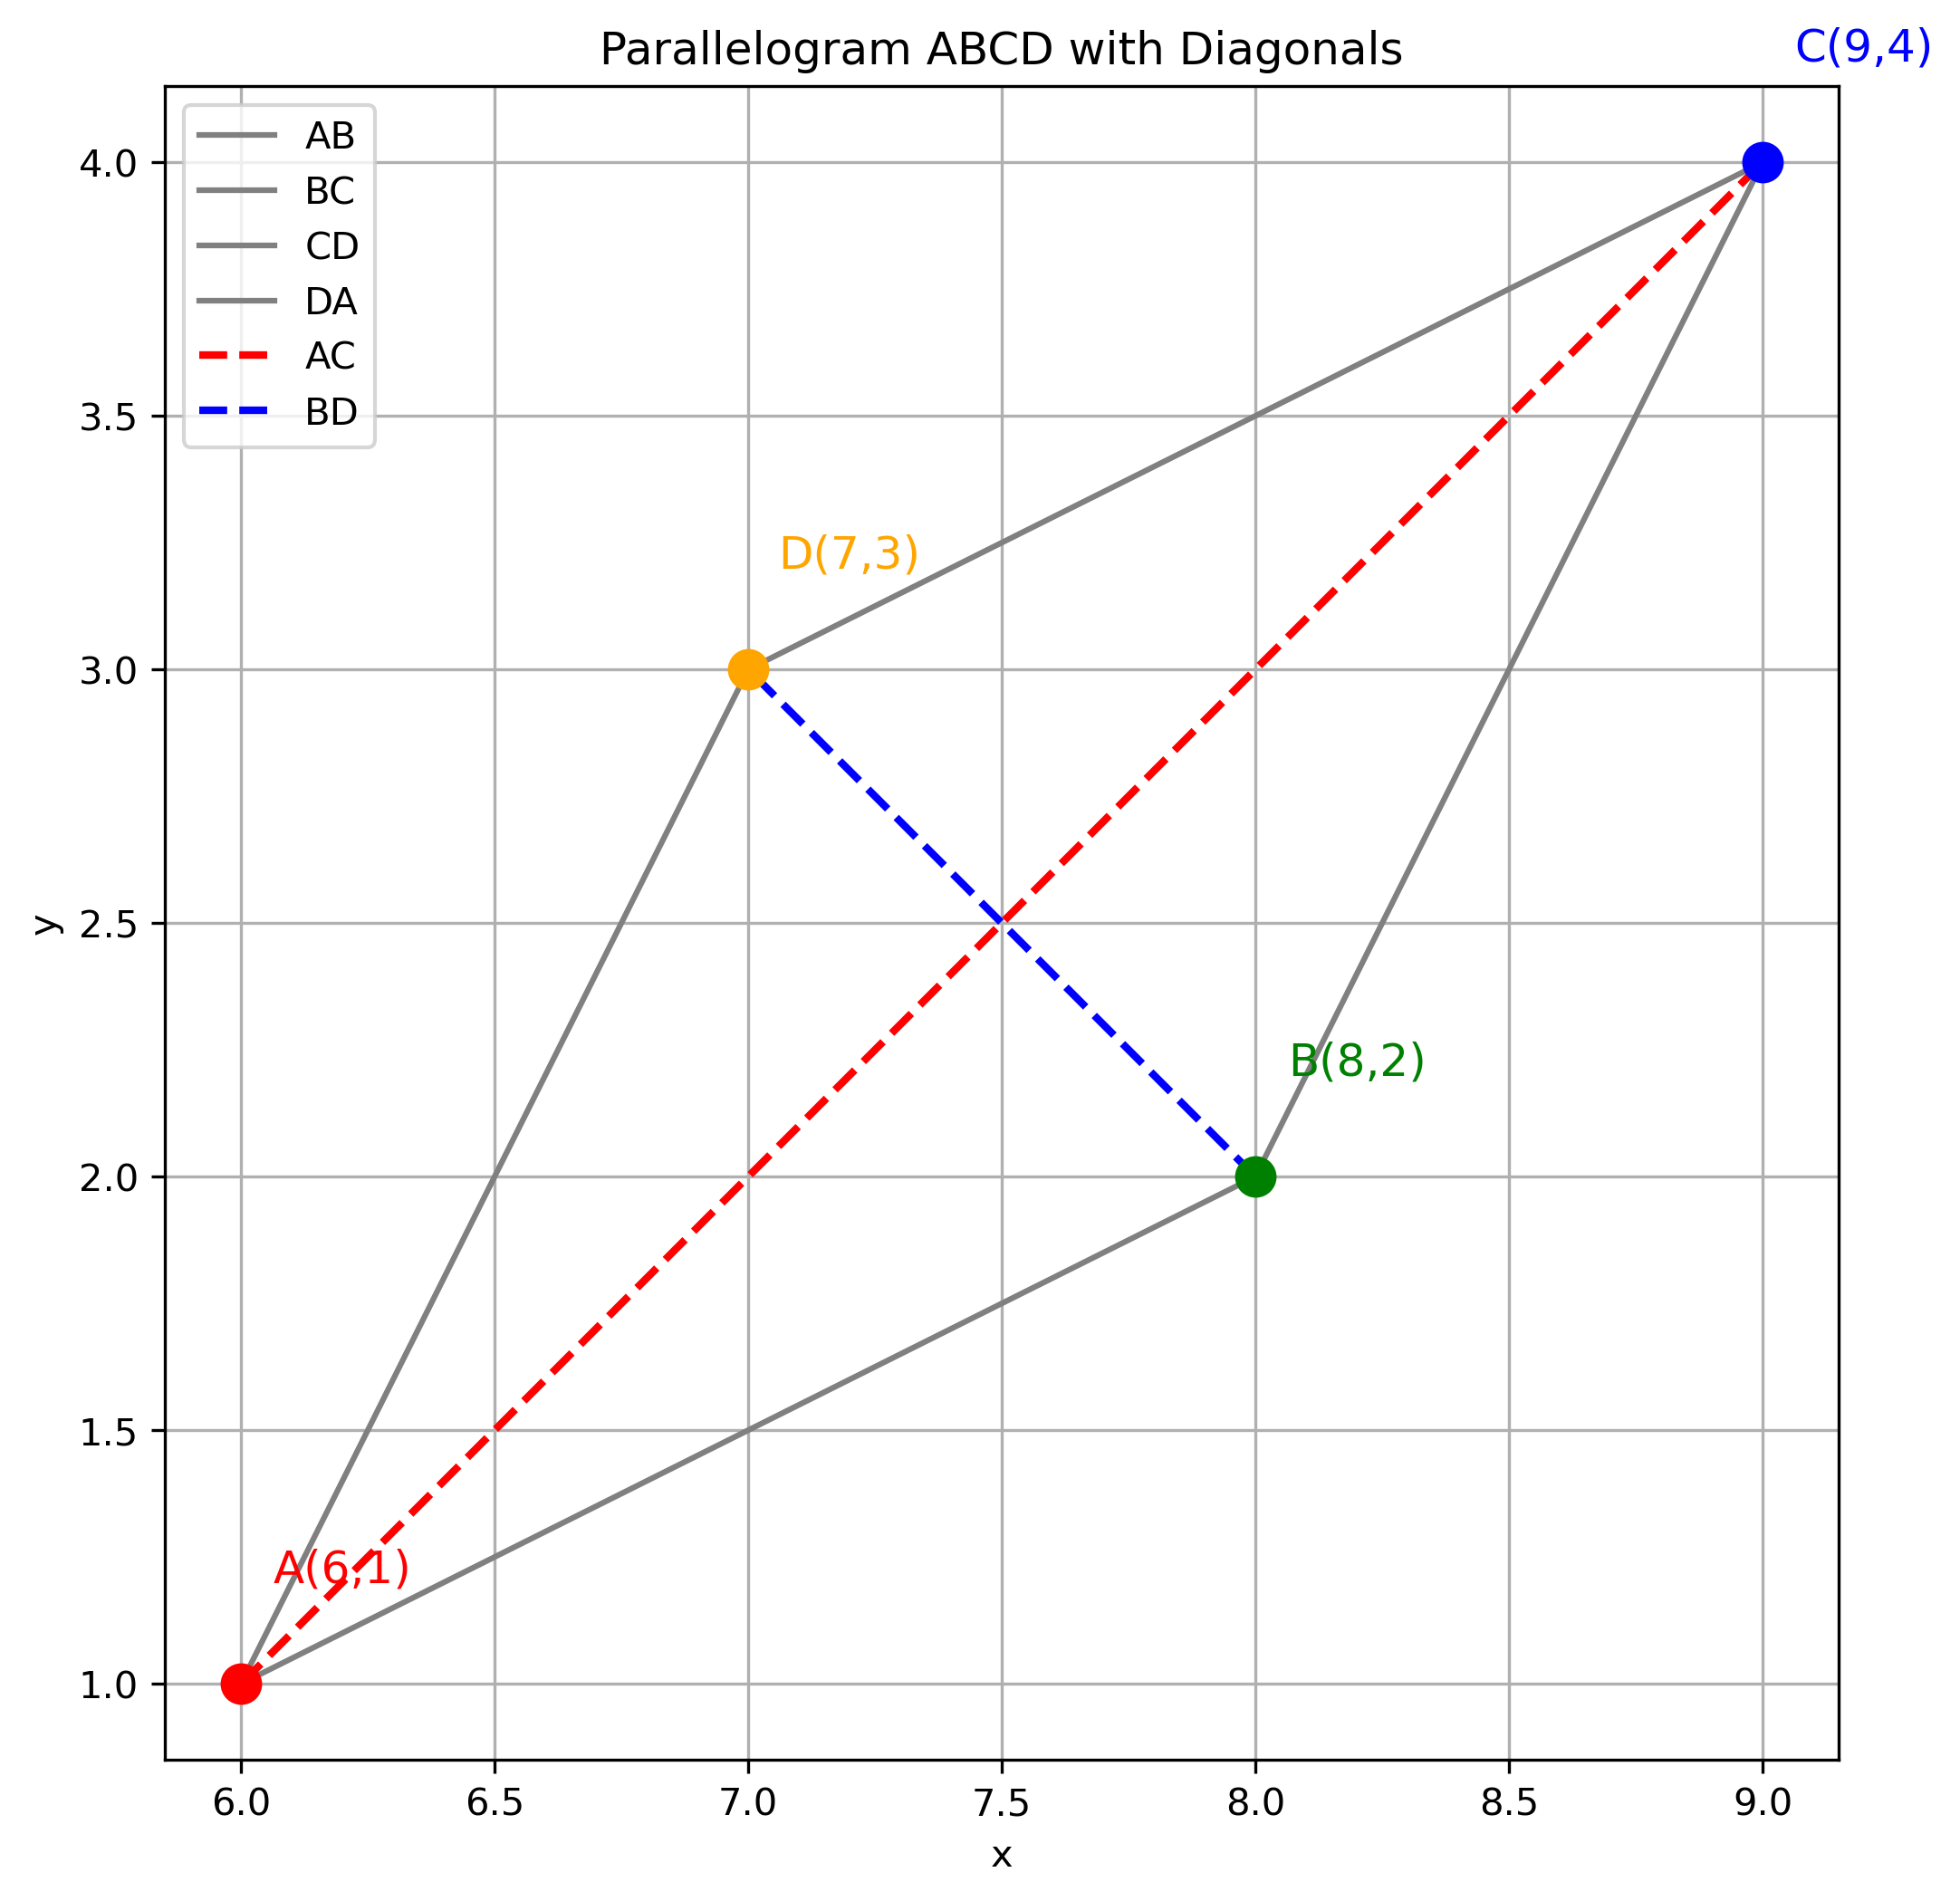
\includegraphics[width=0.4\columnwidth]{Figs/fig1.png}

\caption{graph}
\label{fig:placeholder}
\end{figure}
\begin{enumerate}
\item\hspace{0.5cm}$15:17$
\item\hspace{0.5cm}$16:17$
\item\hspace{0.5cm}$17:15$
\item\hspace{0.5cm}$17:16$\\
 \end{enumerate}
 \hfill $\brak{GATE\ BM\ 2020}$
 \end{enumerate}
 
 \newpage
\maketitle{BM:Biomedical Engineering}\\
  \noindent \textbf{Q. 1 --Q.  \textbf{25}} carry one mark each
\begin{enumerate}

\item m1 and m2 are the roots of the characteristic equation of a linear second order physical system. Match the nature of the roots with the natural response of the system.\\

\begin{center}
\begin{tabular}{|c|l|c|l|}
\hline
\textbf{} & \textbf{Nature of roots} & \textbf{} & \textbf{System response} \\
\hline
P & $m_1$ and $m_2$ are real and distinct & K & Critically damped \\
\hline
Q & $m_1$ and $m_2$ are equal & L & Overdamped \\
\hline
R & $m_1$ and $m_2$ are complex & M & Underdamped \\
\hline
\end{tabular}
\end{center}

\begin{enumerate}
\item\hspace{0.5cm}P-L, Q-M, R-K
\item\hspace{0.5cm}P-M, Q-L, R-K
\item\hspace{0.5cm}P-L, Q-K, R-M
\item\hspace{0.5cm}P-M, Q-K, R-L
\end{enumerate}
 \hfill $\brak{GATE\ BM\ 2020}$

\item A person is sitting in a chair with feet on the ground. While rising up on his feet, the kinematic motion NOT occurring is
\begin{enumerate}[label=\alph*)]
\item\hspace{0.5cm}Hip extension
\item\hspace{0.5cm}Plantar flexion
\item\hspace{0.5cm}Hip flexion
\item\hspace{0.5cm}Knee extension
\end{enumerate}
 \hfill $\brak{GATE\ BM\ 2020}$
 
\item The equipment that measures elasticity of blood vessel in vivo is
\begin{enumerate}[label=\alph*)]
\item\hspace{0.5cm}Rheometer
\item\hspace{0.5cm}Dimension analyser
\item\hspace{0.5cm}Thermomechanical analyser
\item\hspace{0.5cm}Dynamic mechanical analyser
\end{enumerate}
 \hfill $\brak{GATE\ BM\ 2020}$
 
\item Biomaterials with shape memory effects are NOT used in
\begin{enumerate}[label=\alph*)] 
\item\hspace{0.5cm}Intracranial aneurysm clips
\item\hspace{0.5cm}Arterial blood vessel closure devices
\item\hspace{0.5cm}Orthopedic total joint replacements
\item\hspace{0.5cm}Orthodontic dental arch wires
\end{enumerate}
 \hfill $\brak{GATE\ BM\ 2020}$
 
\item The MRI scanner parameter of long TRep or short TEcho will generate a\underline{\hspace{2cm}} contrast image
\begin{enumerate}[label=\alph*)] 
\item\hspace{0.5cm}Proton Density -weighted
\item\hspace{0.5cm}T2- weighted
\item\hspace{0.5cm}T1- weighted
\item\hspace{0.5cm}T2'- weighted
\end{enumerate}
 \hfill $\brak{GATE\ BM\ 2020}$

\item In diagnostic X-ray imaging, the following is NOT a part of primary EM radiation interaction in soft tissue.
\begin{enumerate}[label=\alph*)] 
\item\hspace{0.5cm}Photoelectric effect
\item\hspace{0.5cm}Characteristic radiation production
\item\hspace{0.5cm}Compton scattering
\item\hspace{0.5cm}Pair-production
\end{enumerate}
\hfill $\brak{GATE\ BM\ 2020}$
 
\item 5 MHz ultrasound pulse is used to image a tumor at a depth of 2 cm in a soft tissue. It takes time t for the reflected echo from the tumor to come back to the receiver. Instead, if a 2.5 MHz wave is used, how long will it take for the echo from the same tumor to arrive at the receiver?
\begin{enumerate}[label=\alph*)] 
\item\hspace{0.5cm}$\frac{2}{t}$
\item\hspace{0.5cm}t
\item\hspace{0.5cm}2t
\item\hspace{0.5cm}4t
\end{enumerate}
 \hfill $\brak{GATE\ BM\ 2020}$
 
\item $X(s)$ is a Laplace transform of a signal $x(t)$\\
The Laplace transform of $\frac{dx(t)}{dt}$, assuming $x(0) = 0$, is:
\begin{enumerate}[label=\alph*)] 
\item\hspace{0.5cm}$sX(s)$
\item\hspace{0.5cm}$\frac{X(s)}{s}$
\item\hspace{0.5cm}$\frac{dx(s)}{ds}$
\item\hspace{0.5cm}$\frac{1}{s} \frac{dX(s)}{ds}$
\end{enumerate}
 \hfill $\brak{GATE\ BM\ 2020}$
 
\item Which of the following are odd functions?\\
P: Sin(f)\\
Q: Cos(f)\\
R: Sin(t) + Cos(t)\\
S: Sin(f)Cos(f)\\
\begin{enumerate}[label=\alph*)] 
\item\hspace{0.5cm}Q and S
\item\hspace{0.5cm}P and Q
\item\hspace{0.5cm}P and S
\item\hspace{0.5cm}R and Q
\end{enumerate}
 \hfill $\brak{GATE\ BM\ 2020}$
 
\item State-space model of a system of a model is given as:
\[
\dot{x} = \begin{bmatrix} 0 & 2 \\ a & 0 \end{bmatrix} x + \begin{bmatrix} b \\ 0 \end{bmatrix} u
\]

\[
Y = \begin{bmatrix} 1 & 0 \end{bmatrix} x
\]

The conditions for the system to be controllable are:

\begin{enumerate}[label=(\Alph*)]
    \item\hspace{0.5cm} $a = 0,\ b \ne 0$
    \item\hspace{0.5cm} $a \ne 0,\ b = 0$
    \item\hspace{0.5cm} $a \ne 0,\ b \ne 0$
    \item\hspace{0.5cm} $a = 0,\ b = 0$
\end{enumerate}
 \hfill $\brak{GATE\ BM\ 2020}$

\item In microprocessor systems with memory mapped I/O, which of the following is true?
\begin{enumerate}[label=\alph*)] 
\item\hspace{0.5cm}Only I/O devices with internal memory can be interfaced.
\item\hspace{0.5cm}I/O devices can be accessed using IN and OUT instructions
\item\hspace{0.5cm}Each I/O device can be addressed as a memory location
\item\hspace{0.5cm}Arithmetic and logic operations cannot be directly performed with the I/O data
\end{enumerate}
 \hfill $\brak{GATE\ BM\ 2020}$
 
\item The number of electrodes used in recording standard 12-lead Electrocardiogram (ECG) is
\begin{enumerate}[label=\alph*)] 
\item\hspace{0.5cm}13
\item\hspace{0.5cm}12
\item\hspace{0.5cm}11
\item\hspace{0.5cm}10
\end{enumerate}
 \hfill $\brak{GATE\ BM\ 2020}$
 
\item Which of the following is NOT a part of knee joint?
\begin{enumerate}[label=\alph*)] 
\item\hspace{0.5cm}Patella
\item\hspace{0.5cm}Tibia
\item\hspace{0.5cm}Femur
\item\hspace{0.5cm}Fibula
\end{enumerate}
 \hfill $\brak{GATE\ BM\ 2020}$
 
\item During a routine stethoscopic examination at the left midclavicular-5th intercostal space, murmurs were noted between first and second heart sound. The possible abnormality among the following could be
\begin{enumerate}[label=\alph*)] 
\item\hspace{0.5cm}Aortic stenosis
\item\hspace{0.5cm}Mitral regurgitation
\item\hspace{0.5cm}Mitral stenosis
\item\hspace{0.5cm}Aortic regurgitation
\end{enumerate}
 \hfill $\brak{GATE\ BM\ 2020}$
 
\item The thin filament of a muscle fiber is comprised of
\begin{enumerate}[label=\alph*)] 
\item\hspace{0.5cm}Troponin, Tropomyosin, Actin
\item\hspace{0.5cm}Troponin, Tropomyosin, Titin
\item\hspace{0.5cm}Tropomyosin, Titin, Actin
\item\hspace{0.5cm}Actin, Myosin, Troponin
\end{enumerate}
 \hfill $\brak{GATE\ BM\ 2020}$
 
\item The value of the integral evaluated over the contour C: | z | = 3/2 is \underline{\hspace{2cm}}.\\
\[
\frac{1}{2\pi j} \oint_{ {}{}} \frac{z}{(z - 1)(z - 2)}\, dz
\]  \hfill $\brak{GATE\ BM\ 2020}$

\item The eigenvalues of a 3 x 3 non-singular matrix P are 1, 2 and 3. The trace of matrix \( P^{-1} \) (rounded off to two decimal places) is \underline{\hspace{2cm}}.
 \hfill $\brak{GATE\ BM\ 2020}$
 
\item In a nuclear imaging system, Sodium Iodide (Nal) crystals are used to detect gamma rays of 120 keV. The percentage (\%)
of gamma-rays that will pass through 1 cm of NaI crystal, assuming the Half-Value-Layer (HVL) of Nal as 0.2 cm, is \underline{\hspace{2cm}}.
(rounded off to one decimal place).
 \hfill $\brak{GATE\ BM\ 2020}$
 
\item The distal end of an endoscope is placed at a distance of 1 mm from the
gastrointestinal wall. The refractive indices of the fiber core and cladding are 1.5
and 1.45, respectively.\\
The maximum field of view for the endoscope is \underline{\hspace{2cm}}.(rounded off to one decimal place). \hfill $\brak{GATE\ BM\ 2020}$

\item The distal end of an endoscope is placed at a distance of 1 mm from the
gastrointestinal wall. The refractive indices of the fiber core and cladding are 1.5
and 1.45, respectively.\\
The maximum field of view for the endoscope is  \underline{\hspace{2cm}} degrees
(rounded off to one decimal place)  \hfill $\brak{GATE\ BM\ 2020}$


\item Two inductors with the details given below are wound separately on two identical ring type ferromagnetic cores.
\begin{center}
\begin{tabular}{|c|c|c|c|}
\hline
\textbf{Coil} & \textbf{Number of turns} & \textbf{Gauge of wire} & \textbf{Self-Inductance} \\
\hline
Coil-1 & $N$ & $G$ & $L_1$ \\
\hline
Coil-2 & $2N$ & $G/2$ & $L_2$ \\
\hline
\end{tabular}
\end{center}

The ratio $L_2 / L_1$ is \rule{3cm}{0.15mm}.  \hfill $\brak{GATE\ BM\ 2020}$

\item Two dyes X and Y having concentrations in the ratio 0.25 in identical cuvettes were
subjected to absorption measurements in a spectrophotometer. The estimated ratio
of their absorbance is 0.5. The ratio of their molar extinction coefficients is \underline{\hspace{2cm}}.  \hfill $\brak{GATE\ BM\ 2020}$

\item Hydrolysis of one ATP molecule provides an energy of \underline{\hspace{2cm}} kilo calories (correct up to one decimal place). \hfill $\brak{GATE\ BM\ 2020}$

\item An 830 nm laser Doppler flow meter probe is oriented at an angle of 60° to the flow
axis. If the average flow velocity is 3 cm/s, the magnitude of Doppler shift
frequency (kHz) is \underline{\hspace{2cm}} (rounded off to one decimal place).  \hfill $\brak{GATE\ BM\ 2020}$

\item A $100$ mA single current pulse from a pulse generator is used for artificial pacing of
heart at the right ventricle. If the delivered energy does not exceed the fibrillation
threshold of $300$ uJ, the safe duration of the pulse that could be applied to the tissue
mass having an impedance of 500 2 is \underline{\hspace{2cm}} $\mu$ s.  \hfill $\brak{GATE\ BM\ 2020}$

\noindent \textbf{Q. 26 --Q.  \textbf{55}} carry two mark each

\item The resting potential of a mammalian nerve cell is - 80 mV. A certain drug
administered to the body changes the intracellular K+ concentration from 150
mmol/L to 55 mmol/L. The nearest value of cell membrane potential after the
drug administration, assuming that the external equilibrium of K+ does not get
changed during the event, is \\

(Gas constant = 8.315 J/mol/K, core temperature = 37 C and\\

Faraday constant = 96500 C/mol)
\begin{enumerate}[label=\alph*)] 
\item\hspace{0.5cm}-117 mV
\item\hspace{0.5cm}-18.71 mV
\item\hspace{0.5cm}-53.32 mV
\item\hspace{0.5cm}-141.30 mV
\end{enumerate}
\hfill $\brak{GATE\ BM\ 2020}$

\item The arrangement of four resistors of equal value in the diaphragm of a
physiological pressure measurement catheter is shown below. The applied pressure
is observed to cause an increase in length of resistors R2, R4 and an increase in cross sectional area in R1 and R3. The operation results in an equal change in the values of all four resistors. Which among the configuration given below should be used to connect the resistors to form a Wheatstone bridge so that bridge output voltage is proportional to the change in resistance of individual resistors?\\
\begin{figure}[H]
\centering
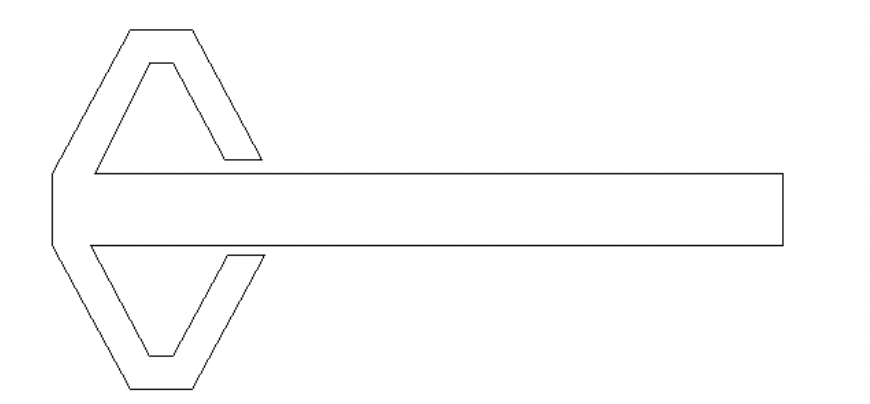
\includegraphics[width=0.4\columnwidth]{Figs/fig2.png}
\label{fig:placeholder}
\end{figure}


\begin{enumerate}[label=\alph*)] 
\item\hspace{0.5cm} I only
\item\hspace{0.5cm} II only
\item\hspace{0.5cm} Neither I nor II
\item\hspace{0.5cm} Both I and II
\end{enumerate}
\hfill $\brak{GATE\ BM\ 2020}$

\item For the given input voltage,\[V_{\text{in}} = 10 \sin\left( 2\pi t \right)
\]to the functional circuit shown below, the output signal will be
\begin{figure}[H]
\centering
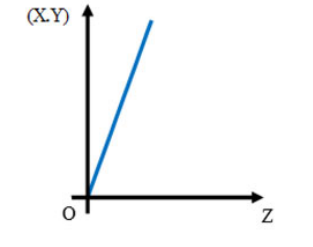
\includegraphics[width=0.4\columnwidth]{Figs/fig3.png}
\caption{functional circuit}
\label{fig:placeholder}
\end{figure}

\begin{figure}[H]
\centering
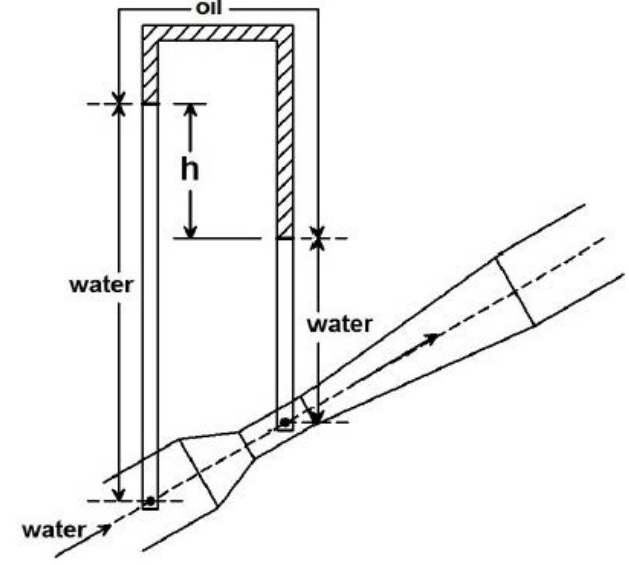
\includegraphics[width=0.4\columnwidth]{Figs/fig7.png}
\caption{options}
\label{fig:placeholder}
\end{figure}
\hfill $\brak{GATE\ BM\ 2020}$

\item During a non-invasive measurement of blood pressure, mean arterial pressure
was observed to be 100 mm Hg. If systolic pressure is 150 mm Hg, the diastolic
pressure would be

\begin{enumerate}[label=\alph*)] 
\item\hspace{0.5cm}110 mm Hg
\item\hspace{0.5cm}75 mm Hg
\item\hspace{0.5cm}70 mm Hg
\item\hspace{0.5cm}50 mm Hg
\end{enumerate} 
\hfill $\brak{GATE\ BM\ 2020}$

\item Two loads are connected to AC supply mains as depicted in the figure. One load
draws 10 kW whereas the other load of 10 kVA is operated at 0.6 pf lagging. To
achieve an overall power factor of 0.9544 lagging, the nearest kVAr rating of the
capacitor bank needed to be connected across the supply mains is equal to 
\begin{figure}[H]
\centering
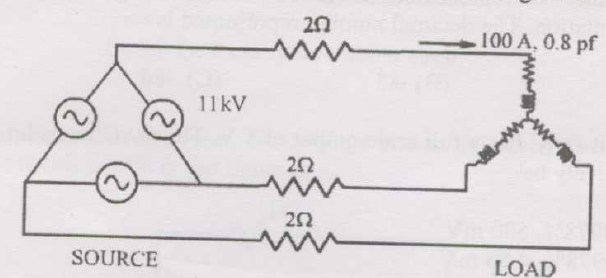
\includegraphics[width=0.4\columnwidth]{Figs/fig4.png}
\caption{AC supply}
\label{fig:placeholder}
\end{figure}

\begin{enumerate}[label=\alph*)] 
\item\hspace{0.5cm}3
\item\hspace{0.5cm}5
\item\hspace{0.5cm}7
\item\hspace{0.5cm}9
\end{enumerate}  
\hfill $\brak{GATE\ BM\ 2020}$

\item The nearest value of power dissipated in the $3~\Omega$ resistance in the circuit is 
\begin{figure}[H]\centering
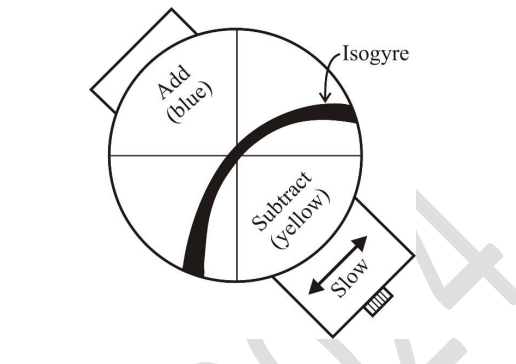
\includegraphics[width=0.4\columnwidth]{Figs/fig5.png}
\caption{circuit}
\label{fig:placeholder}
\end{figure}
\begin{enumerate}[label=\alph*)] 
\item\hspace{0.5cm}3 W
\item\hspace{0.5cm}25/3 W
\item\hspace{0.5cm}12 W
\item\hspace{0.5cm}25/12 W
\end{enumerate} 
\hfill $\brak{GATE\ BM\ 2020}$

\item A second order low pass filter is being constructed by cascading two first order low pass filters with the following transfer functions:  
\[
H_1(\omega) = \frac{1}{1 + j\frac{\omega}{\omega_1}}, 
\quad
H_2(\omega) = \frac{1}{1 + j\frac{\omega}{\omega_2}}
\]
where $\omega_1$ and $\omega_2$ are the respective $-3$ dB cut-off frequencies.The undamped natural frequency $\omega_c$ of the resulting second order low pass filter is  
\begin{enumerate}
    \item[(A)] $\omega_c = \sqrt{\omega_1 \omega_2}$
    \item[(B)] $\omega_c = \omega_1 + \omega_2$
    \item[(C)] $\omega_c = \dfrac{\omega_1 \omega_2}{\omega_1 + \omega_2}$
    \item[(D)] $\omega_c = \sqrt{\omega_1^{2} + \omega_2^{2}}$
\end{enumerate}

 \hfill $\brak{GATE\ BM\ 2020}$

\item Match the bridge type with the application given below:\\
\begin{center}
\begin{tabular}{|c|l|c|l|}
\hline
\textbf{} & \textbf{Name of the bridge} & \textbf{} & \textbf{Application} \\
\hline
P & Maxwell bridge & K & Measurement of Low resistance \\
\hline
Q & Kelvin double bridge & L & Measurement of medium Q-coil inductance \\
\hline
R & Hay bridge & M & Measurement of capacitance \\
\hline
S & Schering bridge & N & Measurement of High Q-coil inductance \\
\hline
\end{tabular}
\end{center}

\begin{enumerate}[label=\alph*)] 
\item\hspace{0.5cm}P-L, Q-K, R-N, S-M
\item\hspace{0.5cm}P-N, Q-K, R-L, S-M
\item\hspace{0.5cm}P-N, Q-L, R-M, S-K
\item\hspace{0.5cm}P-L, Q-M, R-N, S-K
\end{enumerate}
\hfill $\brak{GATE\ BM\ 2020}$

\item For a non-unity feedback system with  
\[
G(s) = \frac{12}{s + 2}
\quad \text{and} \quad
H(s) = \frac{2}{s + 3},
\]
the magnitude of steady-state error to a unit step-input is 

\begin{enumerate}[label=\alph*)] 
\item\hspace{0.5cm}0.45
\item\hspace{0.5cm}0.50
\item\hspace{0.5cm}0.25
\item\hspace{0.5cm}0.20
\end{enumerate}
\hfill $\brak{GATE\ BM\ 2020}$

\item Match the Boolean expression with its minimal realization\\
\begin{center}
\begin{tabular}{|c|c|c|c|}
\hline
\textbf{} & \textbf{Boolean expression} & \textbf{} & \textbf{Minimal realization} \\
\hline
P & $\overline{X}\,\overline{Y}\,\overline{Z} + \overline{X}Y\overline{Z} + \overline{X}YZ$ & K & $X(Y+Z)$ \\
\hline
Q & $XYZ + \overline{X}Y\overline{Z} + XY\overline{Z}$ & L & $\overline{X}(Y+\overline{Z})$ \\
\hline
R & $XY + XYZ + XY\overline{Z} + \overline{X}YZ$ & M & $Z$ \\
\hline
S & $\overline{X}YZ + \overline{X}YZ + \overline{X}Y\overline{Z} + XYZ$ & N & $Y(X+Z)$ \\
\hline
\end{tabular}
\end{center}
\begin{enumerate}[label=\alph*)] 
\item\hspace{0.5cm}P-K, Q-L, R-N, S-M
\item\hspace{0.5cm}P-L, Q-K, R-N, S-M
\item\hspace{0.5cm}P-L, Q-N, R-M, S-K
\item\hspace{0.5cm}P-M, Q-K, R-L, S-N

\end{enumerate} 
 \hfill $\brak{GATE\ BM\ 2020}$
 
\item The glomerulus filtration process of kidney is modeled as a flat membrane with
pores of radius 1 nm and length of pore 60 nm. The viscosity of the fluid is
0.002 Pa s. The aggregate area of the pores makeup 5% of total surface area of
the membrane. The average pressure on the blood side of the membrane is
8000 Pa and on the ultrafiltrate side is 6200 Pa. The total available area of
membrane is 1.5 m2. The nearest value of resulting filtration rate in cm3/min is 
\begin{enumerate}[label=\alph*)] 
\item\hspace{0.5cm}0.14
\item\hspace{0.5cm}1.40
\item\hspace{0.5cm}8.43
\item\hspace{0.5cm}84.37
\end{enumerate}
 \hfill $\brak{GATE\ BM\ 2020}$
 
\item During resting state, the voltage outside the cell membrane compared to that inside the membrane is\underline{\hspace{2cm}}.Under such conditions, the intracellular and extracellular regions have
\underline{\hspace{2cm}} and \underline{\hspace{2cm}} concentrations, respectively.
\begin{enumerate}[label=\alph*)] 
\item\hspace{0.5cm}More positive, more Potassium [K$^+$], more Sodium [Na$^+$]
\item\hspace{0.5cm}More negative, more Potassium [K$^+$], more Sodium [Na$^+$]
\item\hspace{0.5cm}More negative, more Sodium [Na$^+$], more Potassium [K$^+$]
\item\hspace{0.5cm}More positive, more Sodium [Na$^+$], more Potassium [K$^+$]
\end{enumerate}
 \hfill $\brak{GATE\ BM\ 2020}$
 
\item The tensile strength of a degradable suture used for a surgical procedure in the
human body is observed to decrease exponentially from its original strength by
40\% and 50\% after 10 days and 20 days, respectively. The closest approximation
of the time taken for the tensile strength to decay to 20\% of its original value
would be
\begin{enumerate}[label=\alph*)] 
\item\hspace{0.5cm}35 days
\item\hspace{0.5cm}45 days
\item\hspace{0.5cm}60 days
\item\hspace{0.5cm}70 days
\end{enumerate}
 \hfill $\brak{GATE\ BM\ 2020}$
 
\item A 60 kg person is standing on one foot on a force plate. The ground reaction
force is found to act 40 mm anterior to the ankle joint. The mass center of a foot
is 60 mm from the Trochanter Knee Ankle (TKA) line. If the weight of the foot
is 0.8 kg, the closest value of \textbf{magnitude} of moment acting on the ankle joint is
\begin{enumerate}[label=\alph*)] 
\item\hspace{0.5cm}23 Nm
\item\hspace{0.5cm}48 Nm
\item\hspace{0.5cm}235 Nm
\item\hspace{0.5cm}466 Nm
\end{enumerate}
 \hfill $\brak{GATE\ BM\ 2020}$
 
\item The temperature of bone cement is increased from $37^\circ\mathrm{C}$ to $87^\circ\mathrm{C}$ during the

femoral hip arthroplasty. The cement thickness is noted to be 20 mm. The stress
developed due to exothermic reaction of bone cement during the polymerization
process and shrinkage of the bone cement, respectively, are\\

Assume that\\

(i) bone, cement, and implant are modeled as a set of concentric cylinders\\

(ii) no direct adhesion takes place between bone and cement\\

(iii) temperature is uniform\\

Coefficient of thermal expansion of bone cement = $90 \times 10^{-6}\,^\circ\mathrm{C}$\\
Young's modulus of bone cement = 3.5 GPa

\begin{enumerate}[label=\alph*)] 
\item\hspace{0.5cm}15.75 MPa, 90 $\mu$m
\item\hspace{0.5cm}15.75 MPa, 110 $\mu$m
\item\hspace{0.5cm}6.85 MPa, 110 $\mu$m
\item\hspace{0.5cm}6.85 MPa, 90 $\mu$m
 \end{enumerate}
 \hfill $\brak{GATE\ BM\ 2020}$
 
\item A patient is initially imaged in a 1 Tesla MRI scanner and induced voltage is found 
to be equal to $V_1$. The expression for the magnitude of the received voltage in the 
coil is given below.
\[
|V| = 2 \pi \gamma_0 V_S M_0 (\sin \alpha) \beta^r
\]
  
$V_S$: MR slice volume,
$M_0$: Magnitude of resultant magnetic vector,\\
$\gamma_0$: Larmor frequency,  
$\alpha$: tip angle,  
$\beta^r$: Magnetic field sensitivity of receive coil.  \\

When the patient is shifted to a 3 Tesla MRI scanner that uses the same sequence 
and the slice thickness is halved, the magnitude of the induced voltage is found 
to be equal to $V_2$. The ratio $V_2/V_1$ is
\begin{enumerate}[label=\alph*)] 
\item\hspace{0.5cm}1.5
\item\hspace{0.5cm}3.0
\item\hspace{0.5cm}4.5
\item\hspace{0.5cm}6.0
\end{enumerate}
 \hfill $\brak{GATE\ BM\ 2020}$
 
\item A 3 MHz ultrasound transducer transmits a 3-cycle long pulse into a soft tissue at 
normal incidence to fat and liver interface. The axial resolution (mm) and the 
amplitude reflection coefficient at fat-liver interface, respectively, are

\[
c_{\text{tissue}} = 1500 \ \text{m/s}, \quad 
c_{\text{fat}} = 1450 \ \text{m/s}, \quad 
c_{\text{liver}} = 1570 \ \text{m/s},
\]
\[
\rho_{\text{fat}} = 920 \ \text{kg/m}^3, \quad 
\rho_{\text{liver}} = 1060 \ \text{kg/m}^3
\]

\begin{enumerate}[label=\alph*)] 
\item\hspace{0.5cm}0.5, 0.22
\item\hspace{0.5cm}0.75, 0.22
\item\hspace{0.5cm}0.5, 0.11
\item\hspace{0.5cm}0.75, 0.11
\end{enumerate}
 \hfill $\brak{GATE\ BM\ 2020}$
 
\item The forward biased current of a silicon (Si) diode is being calculated from the 
exponential model of the V-I characteristics. If the diode current $I_D = 1 \ \text{mA}$ 
at a voltage drop $V_D = 0.7 \ \text{V}$, the nearest value of $I_D$ when 
$V_D = 0.8 \ \text{V}$ is\\

Assume thermal voltage $V_T = 25.3 \ \text{mV}$ for Si diode.
\begin{enumerate}[label=\alph*)] 
\item\hspace{0.5cm}0.133 mA
\item\hspace{0.5cm}2 mA
\item\hspace{0.5cm}52 mA
\item\hspace{0.5cm}90 mA
\end{enumerate}
 \hfill $\brak{GATE\ BM\ 2020}$
 
\item A continuous random variable $x$ has a probability density function given by  

\[
f(x) = e^{-a|x|} \quad (-\infty < x < \infty)
\]

where $a$ is a real constant. The variance of $x$ is \underline{\hspace{2cm}} 
(correct up to one decimal place). 
\hfill $\brak{GATE\ BM\ 2020}$

\item The magnitude of the gradient of the function 
\[
f(x, y) = x^{2} + y^{2}
\]
at the point $(1,1)$ is \underline{\hspace{2cm}}  (rounded off to two decimal places). \hfill $\brak{GATE\ BM\ 2020}$

\item The value of the following double integral is \underline{\hspace{2cm}} 
(correct up to three decimal places).
\[
\iint\limits_{R} xy \, dx \, dy
\]
where $R$ is the first quadrant of the circle with center at the origin and radius of one unit. \hfill $\brak{GATE\ BM\ 2020}$

\item A gynaecologist recorded the blood pressure (BP) of patients as shown in the 
Table below. Using Regression process, the diastolic BP of a 38 year old patient 
(mm Hg) is \underline{\hspace{2cm}} (rounded off to two decimal places).\\
\begin{center}
\begin{tabular}{|c|c|c|c|c|c|c|c|c|c|}
\hline
\textbf{Age (years)} & 23 & 24 & 25 & 26 & 28 & 29 & 31 & 35 & 40 \\
\hline
\textbf{\begin{tabular}[c]{@{}c@{}}BP (diastolic)\\ mm Hg\end{tabular}} & 65 & 60 & 62 & 70 & 70 & 73 & 75 & 83 & 90 \\
\hline
\end{tabular}
\end{center}
 \hfill $\brak{GATE\ BM\ 2020}$

\item A person in standing position first flexes the hip by 50$^\circ$ from the initial
Trochanter knee ankle (TKA) line and then flexes knee by 20$^\circ$. The distance of ankle joint from the initial TKA line is \underline{\hspace{2cm}} (rounded off to nearest integer).\\
(i)   the distance between hip joint and knee joint is 400 mm\\
(ii)  the distance between knee joint and ankle joint is 300 mm.  \hfill $\brak{GATE\ BM\ 2020}$

\item A chest radiograph of 36 cm x 48 cm is digitized. If we want to preserve details
in the image to a spatial resolution of 6 cycles/mm, the approximate image data size in MB for an 8 bit quantization is \underline{\hspace{2cm}} (rounded of to two decimal places).  \hfill $\brak{GATE\ BM\ 2020}$

\item An X-ray radiography scenario is shown in the figure. If the number of incident 
photons ($N_i$) is equal to $2 \times 10^{6}$ at 50 keV, the number of photons ($N_d$) 
that exit the tissue is \underline{\hspace{2cm}}  $\times 10^{6}$ (rounded off to two decimal places).\\
\begin{figure}[H]
\centering
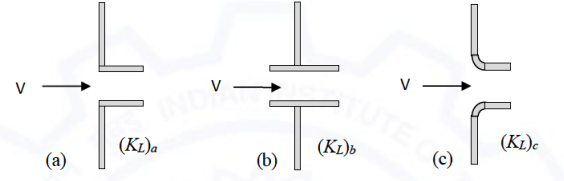
\includegraphics[width=0.4\columnwidth]{Figs/fig6.png}
\caption{radiography}
\label{fig:placeholder}
\end{figure}

(use linear attenuation coefficient for soft tissue and blood at 50 keV as 
$0.4 \ \text{cm}^{-1}$ and $0.2 \ \text{cm}^{-1}$, respectively).  \hfill $\brak{GATE\ BM\ 2020}$

\item The wavelength of an electron accelerated to a potential of 1 V is \underline{\hspace{2cm}}nm 
(rounded off to two decimal places).\\

Mass of electron $= 9.11 \times 10^{-31} \ \text{kg}$\\

Plank's constant, $h = 6.63 \times 10^{-34} \ \text{J.s}$

Charge of electron $= 1.6 \times 10^{-19} \ \text{C}$  \hfill $\brak{GATE\ BM\ 2020}$

\item In a permanent magnetic moving coil (PMMC) instrument having following 
specifications, the angular deflection of the pointer for a coil current of 
$100 \ \mu\text{A}$ will be \underline{\hspace{2cm}} degrees 
(rounded off to one decimal place).\\

Magnetic flux density $= 1.5 \ \text{Tesla}$\\

Torsional spring constant $= 2 \times 10^{-6} \ \text{Nm/deg}$\\

Cross sectional area of the coil $= 2.5 \ \text{cm}^2$\\

Number of turns of the coil $= 500$  \hfill $\brak{GATE\ BM\ 2020}$

\item Arterial blood extracted from a healthy adult showed an oxygen partial pressure 
value of $40 \ \text{mm Hg}$. The total oxygen content in the arterial blood measured 
in \%V/V is \underline{\hspace{2cm}}  (rounded off to one decimal place).\\

Given: Solubility of oxygen in blood $= 0.003 \ \text{ml/mm Hg/dL}$\\

Hemoglobin oxygen saturation $= 95 \ \%$\\

Oxygen carrying capacity of Hb $= 1.34 \ \text{ml/g}$\\

Arterial blood hemoglobin concentration $= 15 \ \text{g/dL}$  \hfill $\brak{GATE\ BM\ 2020}$

\item In the process of measuring blood flow from an artery using C-clamp magnetic 
flow probe, the voltage recorded across diametrically opposite sites of the artery 
is $3.75 \ \text{nV}$. The blood flow rate through the artery is  \underline{\hspace{2cm}}$\text{cm}^3/\text{s}$ 
(rounded off to two decimal places).\\

The inner diameter of the C-clamp $= 0.5 \ \text{cm}$\\

The magnetic flux density $= 1.5 \times 10^{-5} \ \text{Wb/m}^2$
 \hfill $\brak{GATE\ BM\ 2020}$
 
\item A cell is injected with a current $i(t) = u(t)$ to produce a change in the 
intracellular membrane voltage $v(t)$. The cell-membrane is modeled as a 
linear system with impulse response 
\[
h(t) = A e^{-\frac{t}{\tau}} u(t).
\]
The cell membrane voltage output at $5 \ \text{ms}$ is \underline{\hspace{2cm}} mV.\\

Use $A = -34 \ \text{V/s}$; $\tau = 3 \ \text{ms}$.  \hfill $\brak{GATE\ BM\ 2020}$

\newpage
\maketitle{Answer key BM:Biomedical Engineering}

\begin{figure}[H]
\centering
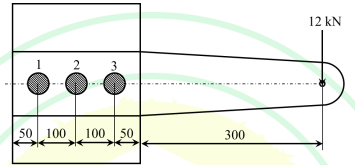
\includegraphics[width=0.4\columnwidth]{Figs/fig8.png}
\caption{key}
\label{fig:placeholder}
\end{figure}

\begin{figure}[H]
\centering
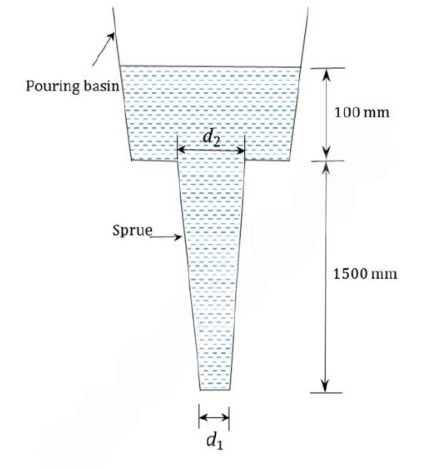
\includegraphics[width=0.4\columnwidth]{Figs/fig9.png}
\caption{key}
\label{fig:placeholder}
\end{figure}




\end{enumerate}

\end{document}
